\documentclass[addpoints]{exam}

\usepackage[utf8]{inputenc}
\usepackage{amsmath,amsthm,amssymb}
\title{Sample Exam}
\author{Param Rathour}
\date{\today}
\usepackage{tikz}
\usepackage{pgfplots}

\begin{document}
\maketitle
\makebox[\textwidth]{Name:\enspace\hrulefill}

\vspace{5mm}

\makebox[\textwidth]{Roll Number:\enspace\hrulefill}

\vspace{2em}

\begin{center}
\combinedgradetable[h][questions]
\end{center}

\vspace{8em}

\begin{center}
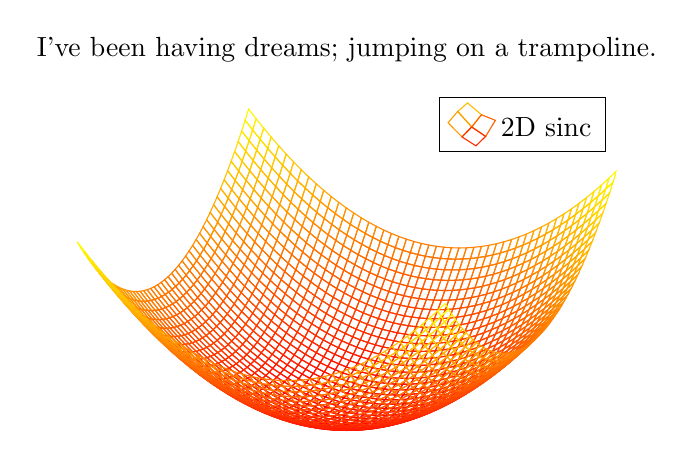
\begin{tikzpicture}
\begin{axis}[
    title=I’ve been having dreams; jumping on a trampoline.,
    hide axis,
    colormap/redyellow,
]
\addplot3[
    mesh,
    samples=50,
    domain=-8:8,
]
{x^2+y^2};
\addlegendentry{$2\text{D sinc}$}
\end{axis}
\end{tikzpicture}
\end{center}
\clearpage
\begin{questions}
\question You need to use \verb!pgfplot! to draw the figure. The source code for this plot is taken from an Overleaf tutorial. Read the tutorial to learn about the functionality of pgfplot, you will eventually find the relevant snippet.
\begin{parts}
\part[5] Play around with the parameters to achieve this trampoline effect.
\part[5] Change the title, and the colour scheme from the original.

\vspace{1mm}
\droptotalpoints
\end{parts}
\question
Read the caption to the figure.
\begin{parts}
\part[3] Which song is the caption taken from?
\part[2] This song is a duet. Who is the male vocalist?
\part[2] Which of the following was he associated with?\\
	\begin{oneparchoices}
		\choice Led Zeppelin
		\choice Queen
		\choice One Direction
		\choice Nirvana
	\end{oneparchoices}
\part[3] Which of the following are Linkin Park songs?
	\begin{checkboxes}
		\choice Faint
		\choice Carnival of Rust
		\choice Enter Sandman
		\choice New Divide
	\end{checkboxes}
\bonuspart[5] In the above question, which artist(s) made the other song(s)?
\vspace{7em}
\end{parts}
\droptotalpoints
\bonusquestion[10] Describe how Green Day’s American Idiot connects with the current sociopolitical climate of the USA.
\end{questions}
\end{document}